While the type graph method~\cite{bruggink2014termination, bruggink2015proving,endrullis2024generalized_arxiv_v2} can prove termination for this example, it requires constructing an appropriate weighted type graph, a task that is difficult in general~\cite[\textsection 6]{bruggink2015proving}. 
In contrast, our criterion only requires checking simpler conditions.
\begin{example}
    \label{subgraph_counting:ex:termination:grsaa}
    Consider the rewriting rule $\rho$ in~\autoref{subgraph_counting:ex:grsaa_rx}, let $X$ be the graph \tikz[baseline=-0.5ex]{
        \node (x) at (0,0) {$\bullet$};
        \node (y) at (1,0) {$\bullet$ }; 
        \node (z) at (2,0) { $\bullet$};
        \draw[->] (x) -- (y) node[midway, above] {$a$};
        \draw[<-] (z) -- (y) node[midway, above] {$a$};
    }, $\mathbb{X} = \{X\}$ and $s_\mathbb{X}(X) = 1$. The rule is $X$-non-increasing as shown in~\autoref{example:grs_aa:has_more_left}. 
    Since \(w_{s_\mathbb{X}}(\operatorname{lhs}(\rho)) = 1 > 0 = w_{s_\mathbb{X}}(\operatorname{rhs}(\rho)) \),
    it terminates by~\autoref{subgraph_counting:thm:termination_grs}.
\end{example}
We consider an example for which the techniques from \cite{bruggink2014termination,bruggink2015proving,endrullis2024generalized_arxiv_v2,plump2018modular,overbeek2024termination_lmcs} fail.
\begin{example} 
    \label{subgraph_counting:ex_contrib_variant}
    The rewriting rule shown in~\autoref{fig:subgraph_counting:ex_confdkjfakljl} is a variant of a rule presented in \cite[Example 6]{plump2018modular}, obtained by removing all edges in the interface:
     
    \begin{figure}[!htbp]
        \centering
        \resizebox{0.6\textwidth}{!}{
            \begin{tikzpicture}
                \graphbox{$L$}{0mm}{0mm}{35mm}{35mm}{2mm}{-5mm}{
                    \coordinate (delta) at (0,-18mm);
                    \node[draw,circle] (l1) at ($(delta) + (-1,1.5)$) {1};
                    \node[draw,circle] (l2) at ($(delta) + (1,1.5)$) {2};
                    \node[draw,circle] (l3) at ($(delta) + (0,0)$) {3};
                    \draw[->] (l1) -- (l3) node[midway,left] {s};
                    \draw[->] (l2) -- (l3) node[midway,right] {s};
                    \draw[->] (l3) edge [loop below] node {0} (l3);
                }
                \graphbox{$K$}{40mm}{0mm}{35mm}{35mm}{2mm}{-5mm}{
                    \coordinate (delta) at (0,-18mm);
                    \coordinate (interfaceorigin) at ($(delta) +(5,0)$);
                    \node[draw,circle] (r1) at ($(delta) +(-1,1.5)$) {1};
                    \node[draw,circle] (r2) at ($(delta) +(0.5,1.5)$) {2};
                    \node[draw,circle] (r3) at ($(delta) + (0,0)$) {3};
                    % \draw[->] (r1) -- (r3) node[midway,left] {s};
                    % \draw[->] (r3) edge [loop below] node {0} (r3);
                }
                \graphbox{$R$}{80mm}{0mm}{50mm}{35mm}{2mm}{-5mm}{
                    \coordinate (delta) at (-10mm,-18mm);
                    \node[draw,circle] (r1) at ($(delta) + (-1,1.5)$) {1};
                    \node[draw,circle] (r2) at ($(delta) + (0.5,1.5)$) {2};
                    \node[draw,circle] (r3) at ($(delta) + (0,0)$) {3};
                    \node[draw,circle] (r4) at ($(delta) + (1,0)$) {4};
                    \draw[->] (r1) -- (r3) node[midway,left] {s};
                    \draw[->] (r2) -- (r4) node[midway,right] {s};
                    \draw[->] (r4) edge [loop below] node {0} (r4);
                    \draw[->] (r3) edge [loop below] node {0} (r3);
                    \node[draw,circle] (r5) at ($(r2) + (1.5,0)$) {};
                    \draw[->] (r5) edge [loop below] node {0} (r5);
                    \draw[->] (r5) edge [loop right] node {0} (r5);
                    \draw[->] (r5) edge [loop left] node {0} (r5);
                }
                % \graphbox{$R_x$}{40mm}{40mm}{35mm}{35mm}{2mm}{-5mm}{
                %     \coordinate (delta) at (0,-18mm);
                %     \coordinate (rxorigin) at ($(interfaceorigin)+(0,6)$);
                %     \node[draw,circle] (r1) at ($(delta) + (-1,1.5)$) {1};
                %     \node[draw,circle] (r2) at ($(delta) +  (0.5,1.5)$) {2};
                %     \node[draw,circle] (r3) at ($(delta) +  (0,0)$) {3};
                %     \draw[->] (r1) -- (r3) node[midway,left] {s};
                %     % \draw[->] (r3) edge [loop below] node {0} (r3);
                % }
                \node () at (38mm,-18mm) {$\leftarrowtail$};
                \node () at (77mm,-18mm) {$\rightarrowtail$};
                % \node () at (57mm,2mm) {$\uparrowtail$};
                % \node () at (38mm,2mm) {$\swarrowtail$};
                % \node () at (79mm,2mm) {$\searrowtail$};
            \end{tikzpicture}
            }
            \caption{}
            \label{fig:subgraph_counting:ex_confdkjfakljl}
    \end{figure}
        %     \caption{Diagram of~\autoref{ex_contrib_variant}}
        %     \label{fig:contrib_variant}
        % \end{figure}
        Let $X$ be the ruler-graph 
        \tikz[baseline=-0.5ex]{ 
                \node (x) at (0,0) {$\bullet$}; 
                \node (y) at (1,0) {$\bullet$};
                \node (z) at (2,0) {$\bullet$};
                \draw[->] (x) -- (y) node[midway, above] {$s$};
                \draw[->] (z) -- (y) node[midway, above] {$s$};
        }, $\mathbb{X} = \{X\}$ and $s_\mathbb{X}(X)=1$.
        The set \( D(R,X) \) consists of two elements $R'_1$:
        \raisebox{2pt}{
            \scalebox{0.7}{\tikz[baseline=-0.5ex]{
            \node [draw,circle] (x) at (0,0) {1};
            \node[draw,circle] (y) at (1,0) {3};
            \draw[->] (x) -- (y) node[midway, above] {$s$};
        }}} and $R'_2$:
        \raisebox{2pt}{
            \scalebox{0.7}{\tikz[baseline=-0.5ex]{
            \node [draw,circle] (z) at (-1,0) {2};
            \node [draw,circle] (x) at (0,0) {1};
            \node[draw,circle] (y) at (1,0) {3};
            \draw[->] (x) -- (y) node[midway, above] {$s$};
        }}}. 
        Each \( R'_i \) admits a unique monomorphism \( h_{R'_i L} \colon R'_i \rightarrowtail L \) preserving interface elements. 
        Therefore, the rule is $X$-non-increasing under $h_{R'_1L}$ and $h_{R'_2L}$. This is because all conditions in~\autoref{subgraph_counting:def:creates_more_x_on_the_left} are satisfied.
        Since \(w_{s_\mathbb{X}}(L) = 1 > 0 = w_{s_\mathbb{X}}(R)\).
        It follows that the system terminates by~\autoref{subgraph_counting:thm:termination_grs}.
\end{example}

The following example demonstrates the usefulness of a weight function that assigns distinct weight to measurements from different ruler-graphs.
\begin{example} 
    \label{ex:overbeek_5d6}
    Consider the rewriting rules presented in \cite[Example 5.6]{overbeek2024termination_lmcs} illustrated in~\autoref{fig:subgraph_counting:ex_overbdfjkahsdfkjfhew}.
    \begin{figure}[!htbp]
          \centering
        \begin{center} 
          $\rho = $\scalebox{0.7}{{
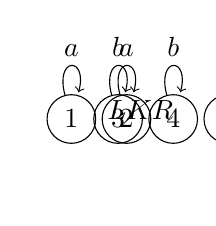
\begin{tikzpicture}[baseline=-10mm]
    \graphbox{$L$}{0mm}{0mm}{31mm}{20mm}{2mm}{-13mm}{
      \node [draw, circle] (x) at (-7mm,0mm) {1};
      \node [draw, circle] (y) at (0mm,0mm) {2};
      \draw[->] (x) edge[loop above] node  {$a$} (x);
      \draw[->] (y) edge [loop above] node {$a$} (y);
    }
    \graphbox{$K$}{32mm}{-0mm}{18mm}{20mm}{0mm}{-10mm}{
    }
    \begin{scope}[opacity=1]        
    \graphbox{$R$}{51mm}{-0mm}{38mm}{20mm}{2mm}{-13mm}{
      \node [draw, circle] (x) at (-7mm,0mm) {3};
      \node [draw, circle] (y) at (0mm,0mm) {4};
      \node [draw, circle] (z) at (7mm,0mm) {5};
      \draw[->] (x) edge[loop above] node  {$b$} (x);
      \draw[->] (y) edge[loop above] node  {$b$} (y);
      \draw[->] (z) edge[loop above] node  {$b$} (z);
    }
    \end{scope}
\end{tikzpicture}
}}
        \end{center}
        \begin{center}
        $\tau = $\scalebox{0.7}{{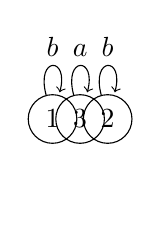
\begin{tikzpicture}[baseline=-10mm]
    \graphbox{L}{0mm}{0}{31mm}{20mm}{2mm}{-13mm}{
        \node[draw,circle] (x) at (-7mm,0mm) {1};
        \node[draw,circle] (y) at (0mm,0mm) {2};
        \draw[->] (x) edge[loop above] node {$b$} (x);
        \draw[->] (y) edge [loop above] node {$b$} (y);
      }
      \graphbox{K}{32mm}{0}{18mm}{20mm}{2mm}{-13mm}{
      }
      \begin{scope}[opacity=1]        
      \graphbox{R}{51mm}{0}{25mm}{20mm}{1mm}{-13mm}{
        \node[draw,circle] (x) at (-3.5mm,0mm) {3};
        \draw[->] (x) edge[loop above] node {$a$} (x);
      }
      \end{scope}
  \end{tikzpicture}}
        }
        \end{center}
        \caption{}
        \label{fig:subgraph_counting:ex_overbdfjkahsdfkjfhew}
  \end{figure}
     Let $X$ be the ruler-graph
    \tikz[baseline=-0.5ex]{
        \node (x) at (0,0) {$\bullet$};
        \draw[->] (x) edge [loop right] node {a} (x);
    }, $Y$ the ruler-graph
    \tikz[baseline=-0.5ex]{
        \node (x) at (0,0) {$\bullet$};
        \draw[->] (x) edge [loop right] node {b} (x);
    } and $\mathbb{X} = \{X, Y\}$.
    The sets $D(R_\rho, X)$, $D(R_\rho, Y)$, $D(R_\tau, X)$ and $D(R_\tau, Y)$ are all empty. Therefore, both rules $\rho$ and $\tau$ are $X$- and $Y$-non-increasing as all conditions in~\autoref{subgraph_counting:def:creates_more_x_on_the_left} are met.
    
    For $s_\mathbb{X}(X) = 5$ and $s_\mathbb{X}(Y) = 3$, we have $
    w_{s_\mathbb{X}}(L_\rho) = 10 > 9 = w_{s_\mathbb{X}}(R_\rho)
    $ and $
    w_{s_\mathbb{X}}(L_\tau) = 6 > 5 = w_{s_\mathbb{X}}(R_\tau)$.
    Therefore, the system terminates by~\autoref{subgraph_counting:thm:termination_grs}.

  However, for $s_\mathbb{X}'(X) = 1$ and $s_\mathbb{X}'(Y) = 1$, we have
    \(
        w_{s_\mathbb{X}'}(L_\rho) = 2 \not > 3 = w_{s_\mathbb{X}'}(R_\rho)
    \) which prevents us from applying~\autoref{subgraph_counting:thm:termination_grs} to prove termination of the rewriting system.
\end{example}

% \begin{example}[Limitation] 
%     \label{ex:plump95_4d1}
%    Consider a rule presented in \cite[Example 4.1]{Plump1995}:
 
%     \begin{center}
%         \resizebox{0.7\textwidth}{!}{
%       $\rho = $  \begin{tikzpicture}[baseline=-20mm]
%         \graphbox{$L$}{0mm}{0}{32mm}{40mm}{0}{0}{
%             \node[draw,circle]  (n1) at (0,-6mm) {1};
%             \node[draw,circle]   (n2) at (0mm,-26mm) {2};
%             \node[draw,circle]   (n3) at (-10mm,-26mm) {3};
%             \node[draw,circle]   (n4) at (10mm,-26mm) {4};
%             \draw[->]  (n2) edge [loop below] node  {a} (n2);
%             \draw[->]  (n3) edge [loop below] node  {b} (n3);
%             \draw[->]  (n1) to node [right] {f} (n2) ;
%             \draw[->]  (n1) to node [right] {f}  (n3);
%             \draw[->]  (n1) to node [right] {f}  (n4);
%           }
%           \graphbox{$K$}{33mm}{0}{32mm}{40mm}{0}{-0}{
%             \node[draw,circle]  (n1) at (0,-6mm) {1};
%             \node[draw,circle]   (n2) at (0mm,-26mm) {2};
%             \node[draw,circle]   (n3) at (-10mm,-26mm) {3};
%             \node[draw,circle]   (n4) at (10mm,-26mm) {4};
%             \draw[->]  (n2) edge [loop below] node  {a} (n2);
%             \draw[->]  (n3) edge [loop below] node  {b} (n3);
%           }
%           \graphbox{$R$}{66mm}{0}{32mm}{40mm}{0}{-0}{
%             \node[draw,circle]  (n1) at (0,-6mm) {1};
%             \node[draw,circle]   (n2) at (0mm,-26mm) {2};
%             \node[draw,circle]   (n3) at (-10mm,-26mm) {3};
%             \node[draw,circle]   (n4) at (10mm,-26mm) {4};
%             \draw[->]  (n2) edge [loop below] node  {a} (n2);
%             \draw[->]  (n3) edge [loop below] node  {b} (n3);
%             \draw[->]  (n1) edge [bend left] node [right] {f} (n4) ;
%             \draw[->]  (n1) edge [bend right] node [left] {f}  (n4);
%             \draw[->]  (n1) to node [right] {f}  (n4);
%           }   
%     \end{tikzpicture}
%         }
%   \end{center}
%   \noindent
%   \begin{minipage}{0.7\textwidth}
%     To prove its termination with our method, a ruler-graph $X$ containing an edge labeled by $f$ must be used, because the number of occurrences of every graph containing only edges labeled by $a$ and $b$ does not change by any rewriting step using $\rho$. But in this case, condition \eqref{def:non_increasing:edge_injective} of~\autoref{def:creates_more_x_on_the_left} cannot be satisfied.
%   \end{minipage}
%   \begin{minipage}{0.3\textwidth}
%     \hfill
%   \begin{center}
%     \begin{tikzpicture} 
%         \graphbox{}{0}{0}{30mm}{20mm}{-10mm}{-10mm}{
%             \node[draw,circle]  (n1) at (0,0mm) {1};
%             % \node[draw,circle]   (n2) at (0mm,-26mm) {2};
%             % \node[draw,circle]   (n3) at (-10mm,-26mm) {3};
%             \node[draw,circle]   (n4) at (20mm,0mm) {4};
%             % \draw[->]  (n2) edge [loop below] node  {a} (n2);
%             % \draw[->]  (n3) edge [loop below] node  {b} (n3);
%             \draw[->]  (n1) edge [bend left] node [above] {f} (n4) ;
%             \draw[->]  (n1) edge [bend right] node [below] {f}  (n4);
%             \draw[->]  (n1) to node {f}  (n4);
%           }  
%     \end{tikzpicture}
%   \end{center}
% \end{minipage}
  
%   \end{example}
% Finally, we present a limitation of our approach.


\begin{example}
  \label{ex_endrullis_6d3_endrullis_5d8}
  Consider the rule presented in~\cite[Example 6.3]{endrullis2024generalized_arxiv_v2} shown in~\autoref{fig:subgraph_counting:ex_endrullis_6d3_endrullis_5d8}.
  \begin{figure}[!htbp]
      \centering
      \resizebox{0.6\textwidth}{!}{
          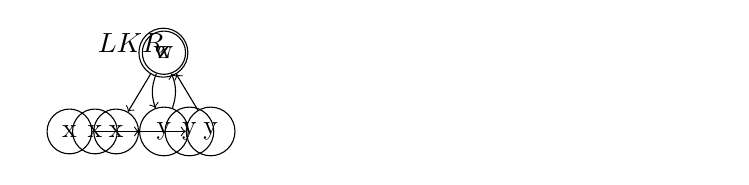
\begin{tikzpicture}
              \graphbox{$L$}{0mm}{0mm}{35mm}{25mm}{2mm}{-8mm}{
                  \coordinate (delta) at (0,-18mm);
                  \node[draw,circle] (x) at (-6mm,-10mm) {x};
                  \node[draw,circle] (y) at (6mm,-10mm) {y};
                  \node[draw,circle]  (z) at (6mm,0mm) {z};
                  \draw[->]  (x) to (y);
                  \draw[->] (y) to[bend right=20] (z);
                  \draw[->]  (z) to[bend right=20] (y);
              }
              \graphbox{$K$}{40mm}{0mm}{35mm}{25mm}{2mm}{-8mm}{
                  \node[draw,circle]  (x) at (-6mm,-10mm) {x};
                  \node[draw,circle]  (y) at (6mm,-10mm) {y};
              }
              \graphbox{$R$}{80mm}{0mm}{35mm}{25mm}{2mm}{-8mm}{
                  \node[draw,circle]  (x) at (-6mm,-10mm) {x};
                      \node[draw,circle]  (y) at (6mm,-10mm) {y};
                      \node[draw,circle]  (z) at (0mm,0mm) {w};
                      \draw[->]  (x) to (y);
                      \draw[->]  (y) to [bend left=0] (z);
                      \draw[->]  (z) to [bend left=0] (x);
              }
              % \graphbox{$R_x$}{40mm}{20mm}{35mm}{15mm}{2mm}{2mm}{
              %     \node[draw,circle]  (x) at (-6mm,-10mm) {x};
              %     \node[draw,circle]  (y) at (6mm,-10mm) {y};
              %     \draw[->]  (x) to (y);
              % }
              \node () at (37mm,-12mm) {$\leftarrowtail$};
              \node () at (78mm,-12mm) {$\rightarrowtail$};
              % \node () at (57mm,2mm) {$\uparrowtail$};
              % \node () at (38mm,2mm) {$\swarrowtail$};
              % \node () at (79mm,2mm) {$\searrowtail$};
          \end{tikzpicture}
      }
      \caption{}
      \label{fig:subgraph_counting:ex_endrullis_6d3_endrullis_5d8}
  \end{figure}

  Let $X$ be the graph 
  \tikz[baseline=-0.5ex]{
      \node (x) at (0,0) {$\bullet$};
      \node (y) at (1,0) {$\bullet$};
      \draw[->] (x) to[bend right=20] (y);
      \draw[->] (y) to[bend right=20] (x); 
  } and $\mathbb{X} = \{X\}$. Let $s_\mathbb{X}$ be the weight function associating the weight of $1$ to $X$. There is only one element 
  \scalebox{0.7}{\tikz[baseline=-0.5ex]{
          \node [draw,circle] (x) at (0,0) {x};
          \node[draw,circle] (y) at (1,0) {y};
          \draw[->] (x) -- (y) node[midway, above] {};
      }}
  in $D(X, R)$. 
   Since $w_{s_\mathbb{X}}(L) = 1 > 0 = w_{s_\mathbb{X}}(R)
      $, the rule terminates by~\autoref{subgraph_counting:thm:termination_grs}.
\end{example}


\begin{example} 
  \label{ex:overbeek_5d5}
  Consider the rewriting rule presented in~\cite[Example 5.5]{overbeek2024termination_lmcs} shown in~\autoref{fig:subgraph_counting:overbeek_5d5}.
  % \begin{figure}[H] 
  %     \center
  \begin{figure}[!htbp]
    \centering
      \resizebox{0.6\textwidth}{!}{
          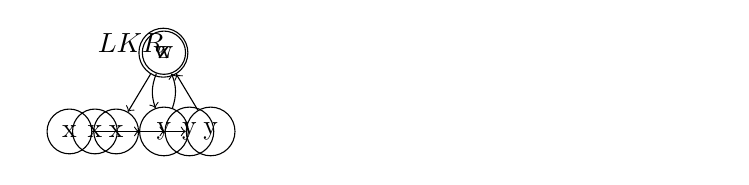
\begin{tikzpicture}
              \graphbox{$L$}{0mm}{0mm}{35mm}{25mm}{2mm}{-8mm}{
                  \coordinate (delta) at (0,-18mm);
                  \node[draw,circle] (x) at (-6mm,-10mm) {x};
                  \node[draw,circle] (y) at (6mm,-10mm) {y};
                  \node[draw,circle]  (z) at (6mm,0mm) {z};
                  \draw[->]  (x) to (y);
                  \draw[->] (y) to[bend right=20] (z);
                  \draw[->]  (z) to[bend right=20] (y);
              }
              \graphbox{$K$}{40mm}{0mm}{35mm}{25mm}{2mm}{-8mm}{
                  \node[draw,circle]  (x) at (-6mm,-10mm) {x};
                  \node[draw,circle]  (y) at (6mm,-10mm) {y};
                  \draw[->] (x) to (y);
              }
              \graphbox{$R$}{80mm}{0mm}{35mm}{25mm}{2mm}{-8mm}{
                  \node[draw,circle]  (x) at (-6mm,-10mm) {x};
                      \node[draw,circle]  (y) at (6mm,-10mm) {y};
                      \node[draw,circle]  (z) at (0mm,0mm) {w};
                      \draw[->]  (x) to (y);
                      \draw[->]  (y) to [bend left=0] (z);
                      \draw[->]  (z) to [bend left=0] (x);
              }
              % \graphbox{$R_x$}{40mm}{20mm}{35mm}{15mm}{2mm}{2mm}{
              %     \node[draw,circle]  (x) at (-6mm,-10mm) {x};
              %     \node[draw,circle]  (y) at (6mm,-10mm) {y};
              %     \draw[->]  (x) to (y);
              % }
              \node () at (37mm,-12mm) {$\leftarrowtail$};
              \node () at (78mm,-12mm) {$\rightarrowtail$};
              % \node () at (57mm,2mm) {$\uparrowtail$};
              % \node () at (38mm,2mm) {$\swarrowtail$};
              % \node () at (79mm,2mm) {$\searrowtail$};
          \end{tikzpicture}
      }
      \caption{}
      \label{fig:subgraph_counting:overbeek_5d5}
  \end{figure}
  %     \caption{Diagram of~\autoref{ex_overbeek}}
  %     \label{fig:overbeek}
  % \end{figure}
    Its termination in the DPO rewriting framework with monic matches can be proved by our approach using the same argument for~\autoref{ex_endrullis_6d3_endrullis_5d8}. 
\end{example}

\begin{example}
  \label{ex:plump_ex4}
  Our method cannot prove the termination of the DPO rewriting system with monic matches presented in~\cite[Example 4]{plump2018modular} shown in~\autoref{fig:subgraph_counting:ex_plump_ex4}.
  \begin{figure}[!htbp]
\begin{center}
  $r_1 = ${ 
   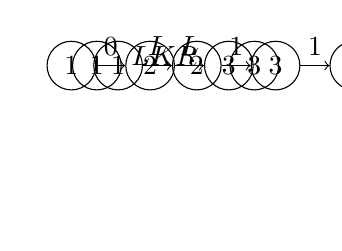
\begin{tikzpicture}[baseline=-20mm]
         \graphbox{$L$}{0mm}{-11mm}{35mm}{15mm}{0.5mm}{-9mm}{
           \node [draw, circle] (x) at (-10mm,0mm) {1};
           \node [draw, circle] (y) at (0mm,0mm) {2};
           \node [draw, circle] (z) at (10mm,0mm) {3};
           \draw[->] (x) to node [above] {$0$} (y);
           \draw[->] (y) to node [above] {$L$} (z);
         }
         \graphbox{$K$}{36mm}{-11mm}{35mm}{15mm}{0.5mm}{-9mm}{
           \node [draw, circle] (x) at (-10mm,0mm) {1};
           %\node [draw, circle] (y) at (0mm,0mm) {2};
           \node [draw, circle] (z) at (10mm,0mm) {3};
         }
         \begin{scope}[opacity=1]        
         \graphbox{$R$}{72mm}{-11mm}{40mm}{15mm}{-4mm}{-9mm}{
           \node [draw, circle] (x) at (-10mm,0mm) {1};
           \node [draw, circle] (y) at (0mm,0mm) {2};
           \node [draw, circle] (z) at (10mm,0mm) {3};
           \node [draw, circle] (w) at (20mm,0mm) {3};
           \draw[->] (x) to node [above] {$L$} (y);
           \draw[->] (y) to node [above] {$1$} (z);
           \draw[->] (z) to node [above] {$1$} (w);
         }
         \end{scope}
       \end{tikzpicture}
  }
 \end{center}
 
 \begin{center}
   $r_2 = ${ 
    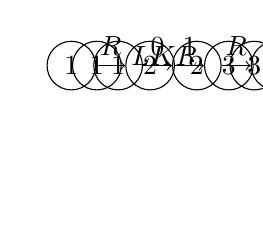
\begin{tikzpicture}[baseline=-20mm]
       \graphbox{$L$}{0mm}{-11mm}{35mm}{15mm}{0.5mm}{-9mm}{
           \node [draw, circle] (x) at (-10mm,0mm) {1};
           \node [draw, circle] (y) at (0mm,0mm) {2};
           \node [draw, circle] (z) at (10mm,0mm) {3};
           \draw[->] (x) to node [above] {$R$} (y);
           \draw[->] (y) to node [above] {$1$} (z);
       }
       \graphbox{$K$}{36mm}{-11mm}{35mm}{15mm}{0.5mm}{-9mm}{
           \node [draw, circle] (x) at (-10mm,0mm) {1};
           %\node [draw, circle] (y) at (0mm,0mm) {2};
           \node [draw, circle] (z) at (10mm,0mm) {3};
       }
       \begin{scope}[opacity=1]        
       \graphbox{$R$}{72mm}{-11mm}{35mm}{15mm}{0.5mm}{-9mm}{
           \node [draw, circle] (x) at (-10mm,0mm) {1};
           \node [draw, circle] (y) at (0mm,0mm) {2};
           \node [draw, circle] (z) at (10mm,0mm) {3};
           \draw[->] (x) to node [above] {$0$} (y);
           \draw[->] (y) to node [above] {$R$} (z);
       }
       \end{scope}
       \end{tikzpicture}
   }
   \end{center}

\begin{center}
  $r_3 = ${ 
   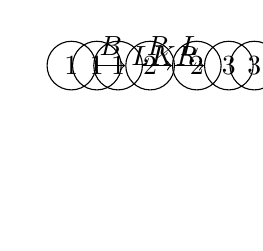
\begin{tikzpicture}[baseline=-20mm]
         \graphbox{$L$}{0mm}{-11mm}{35mm}{15mm}{0.5mm}{-9mm}{
           \node [draw, circle] (x) at (-10mm,0mm) {1};
           \node [draw, circle] (y) at (0mm,0mm) {2};
           \node [draw, circle] (z) at (10mm,0mm) {3};
           \draw[->] (x) to node [above] {$B$} (y);
           \draw[->] (y) to node [above] {$L$} (z);
         }
         \graphbox{$K$}{36mm}{-11mm}{35mm}{15mm}{0.5mm}{-9mm}{
           \node [draw, circle] (x) at (-10mm,0mm) {1};
           %\node [draw, circle] (y) at (0mm,0mm) {2};
           \node [draw, circle] (z) at (10mm,0mm) {3};
         }
         \begin{scope}[opacity=1]        
         \graphbox{$R$}{72mm}{-11mm}{35mm}{15mm}{0.5mm}{-9mm}{
           \node [draw, circle] (x) at (-10mm,0mm) {1};
           \node [draw, circle] (y) at (0mm,0mm) {2};
           \draw[->] (x) to node [above] {$R$} (y);
         }
         \end{scope}
       \end{tikzpicture}
  }
 \end{center}
 
 \begin{center}
   $r_4 = ${ 
    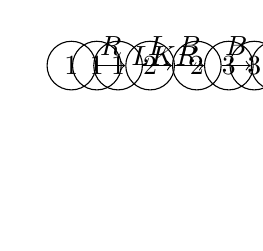
\begin{tikzpicture}[baseline=-20mm]
       \graphbox{$L$}{0mm}{-11mm}{35mm}{15mm}{0.5mm}{-9mm}{
           \node [draw, circle] (x) at (-10mm,0mm) {1};
           \node [draw, circle] (y) at (0mm,0mm) {2};
           \node [draw, circle] (z) at (10mm,0mm) {3};
           \draw[->] (x) to node [above] {$R$} (y);
           \draw[->] (y) to node [above] {$B$} (z);
       }
       \graphbox{$K$}{36mm}{-11mm}{35mm}{15mm}{0.5mm}{-9mm}{
           \node [draw, circle] (x) at (-10mm,0mm) {1};
           %\node [draw, circle] (y) at (0mm,0mm) {2};
           \node [draw, circle] (z) at (10mm,0mm) {3};
       }
       \begin{scope}[opacity=1]        
       \graphbox{$R$}{72mm}{-11mm}{35mm}{15mm}{0.5mm}{-9mm}{
           \node [draw, circle] (x) at (-10mm,0mm) {1};
           \node [draw, circle] (y) at (0mm,0mm) {2};
           \node [draw, circle] (z) at (10mm,0mm) {3};
           \draw[->] (x) to node [above] {$L$} (y);
           \draw[->] (y) to node [above] {$B$} (z);
       }
       \end{scope}
       \end{tikzpicture}
   }
   \end{center}
   \caption{}
   \label{fig:subgraph_counting:ex_plump_ex4}
  \end{figure}
  The rule $r_3$ can be eliminated by considering occurrences of \tikz[baseline=-0.5ex]{
    \node (x) at (0,0) {$\bullet$};
    \node (y) at (1,0) {$\bullet$ };
    \draw[->] (x) -- (y) node[midway, above] {$B$};
  }, and the rule $r_4$ can be eliminated by considering occurrences of \tikz[baseline=-0.5ex]{
  \node (x) at (0,0) {$\bullet$};
  \node (y) at (1,0) {$\bullet$ };
  \draw[->] (x) -- (y) node[midway, above] {$R$};
}.

But our method cannot eliminate $r_1$ and $r_2$. However, combined with the technique proposed by Plump in~\cite{plump2018modular}, we can prove the termination of this rewriting system: $\{r_1\}$ and $\{r_2\}$ are both terminating, and their union is terminating by~\cite{plump2018modular}.
\end{example}


\begin{example}
  \label{ex:overbeek_5d8_plump1995_3d8_plump2018_3_overbeek_5d8}
  Consider the DPO rewriting system presented in~\cite[Example 3.8]{plump1995ontermination} shown in~\autoref{fig:subgraph_counting:overbeek_5d8_plump1995_3d8_plump2018_3_overbeek_5d8}.

  \begin{figure}[!htbp]
    \centering
\begin{center}
 $\rho = ${ 
  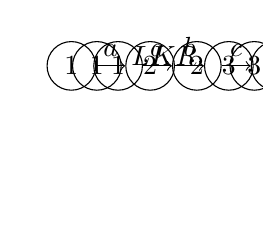
\begin{tikzpicture}[baseline=-20mm]
        \graphbox{$L$}{0mm}{-11mm}{35mm}{15mm}{0.5mm}{-9mm}{
          \node [draw, circle] (x) at (-10mm,0mm) {1};
          \node [draw, circle] (y) at (0mm,0mm) {2};
          \node [draw, circle] (z) at (10mm,0mm) {3};
          \draw[->] (x) to node [above] {$a$} (y);
          \draw[->] (y) to node [above] {$b$} (z);
        }
        \graphbox{$K$}{36mm}{-11mm}{35mm}{15mm}{0.5mm}{-9mm}{
          \node [draw, circle] (x) at (-10mm,0mm) {1};
          %\node [draw, circle] (y) at (0mm,0mm) {2};
          \node [draw, circle] (z) at (10mm,0mm) {3};
        }
        \begin{scope}[opacity=1]        
        \graphbox{$R$}{72mm}{-11mm}{35mm}{15mm}{0.5mm}{-9mm}{
          \node [draw, circle] (x) at (-10mm,0mm) {1};
          \node [draw, circle] (y) at (0mm,0mm) {2};
          \node [draw, circle] (z) at (10mm,0mm) {3};
          \draw[->] (x) to node [above] {$a$} (y);
          \draw[->] (y) to node [above] {$c$} (z);
        }
        \end{scope}
      \end{tikzpicture}
 }
\end{center}

\begin{center}
  $\tau = ${ 
   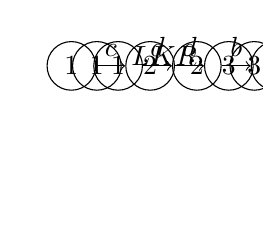
\begin{tikzpicture}[baseline=-20mm]
      \graphbox{$L$}{0mm}{-11mm}{35mm}{15mm}{0.5mm}{-9mm}{
          \node [draw, circle] (x) at (-10mm,0mm) {1};
          \node [draw, circle] (y) at (0mm,0mm) {2};
          \node [draw, circle] (z) at (10mm,0mm) {3};
          \draw[->] (x) to node [above] {$c$} (y);
          \draw[->] (y) to node [above] {$d$} (z);
      }
      \graphbox{$K$}{36mm}{-11mm}{35mm}{15mm}{0.5mm}{-9mm}{
          \node [draw, circle] (x) at (-10mm,0mm) {1};
          %\node [draw, circle] (y) at (0mm,0mm) {2};
          \node [draw, circle] (z) at (10mm,0mm) {3};
      }
      \begin{scope}[opacity=1]        
      \graphbox{$R$}{72mm}{-11mm}{35mm}{15mm}{0.5mm}{-9mm}{
          \node [draw, circle] (x) at (-10mm,0mm) {1};
          \node [draw, circle] (y) at (0mm,0mm) {2};
          \node [draw, circle] (z) at (10mm,0mm) {3};
          \draw[->] (x) to node [above] {$d$} (y);
          \draw[->] (y) to node [above] {$b$} (z);
      }
      \end{scope}
      \end{tikzpicture}
  }
  \end{center}
  \caption{}
  \label{fig:subgraph_counting:overbeek_5d8_plump1995_3d8_plump2018_3_overbeek_5d8}
\end{figure}
  Let $X$ be  \tikz[baseline=-0.5ex]{
      \node (x) at (0,0) {$\bullet$};
      \node (y) at (1,0) {$\bullet$ };
      \node (z) at (2,0) { $\bullet$};
      \draw[->] (x) -- (y) node[midway, above] {$a$};
      \draw[<-] (z) -- (y) node[midway, above] {$b$};
  } 
  We have $D(R_\rho,X) = \emptyset$ and $D(R_\tau,X) = \emptyset$. Therefore, both rules are $X$-non-increasing. 
  We have 
  $|\operatorname{Mono}(X,L)| = 1 > 0 = |\operatorname{Mono}(X,R)|$ for $\rho$, and 
  $|\operatorname{Mono}(X,L)| = 0 = 0 = |\operatorname{Mono}(X,R)|$ for $\tau$, therefore $\rho$ can be eliminated.
  
  Let $Y$ be  \tikz[baseline=-0.5ex]{
      \node (x) at (0,0) {$\bullet$};
      \node (y) at (1,0) {$\bullet$ };
      \draw[->] (x) -- (y) node[midway, above] {$c$};
  }. We have $D(R_\tau,Y) = \emptyset$. Therefore, $\tau$ is $Y$-non-increasing. Moreover, we have $|\operatorname{Mono}(Y,L)| = 1 > 0 = |\operatorname{Mono}(Y,R)|$.
  Thus, this rewriting systems terminates by~\autoref{subgraph_counting:thm:termination_grs}.
\end{example} 


\begin{example}
  \label{ex:overbeek_5d3}
  Consider the rewriting rules presented in~\cite[Example 5.3]{overbeek2024termination_lmcs} shown in~\autoref{fig:subgraph_counting:ex_overbeek_5d3}.
  \begin{figure}[!htbp]
    \centering
\begin{center}
  $\rho = ${ 
  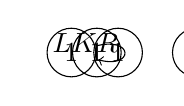
\begin{tikzpicture} 
      \graphbox{$L$}{0mm}{0mm}{23mm}{12mm}{2mm}{-5mm}{
          \node[draw,circle] (x) at (0mm,0mm) {1};
          \draw[->] (x) edge [loop right] node {} (x);
      }
      \graphbox{$K$}{24mm}{0mm}{23mm}{12mm}{2mm}{-5mm}{
        \node[draw,circle] (x) at (0mm,0mm) {1};
      }
      \begin{scope}[opacity=1]        
      \graphbox{$R$}{48mm}{0mm}{30mm}{12mm}{-1mm}{-5mm}{
        \node[draw,circle] (x) at (0mm,0mm) {1};
        \node[draw,circle] (y) at (10mm,0mm) {2};
      }
      \end{scope}
    \end{tikzpicture}
  }
  \end{center}

  \begin{center}
  $\tau = $
  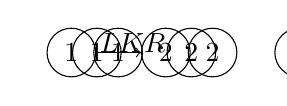
\begin{tikzpicture}
      \graphbox{$L$}{0mm}{-11mm}{32mm}{12mm}{2mm}{-8mm}{
      \node[draw,circle]  (x) at (-6mm,0mm) {1};
      \node[draw,circle] (y) at (6mm,0mm) {2};
      \draw[->]  (x) to (y);
      }
      \graphbox{$K$}{33mm}{-11mm}{32mm}{12mm}{2.5mm}{-8mm}{
          \node[draw,circle]  (x) at (-6mm,0mm) {1};
          \node[draw,circle]  (y) at (6mm,0mm) {2};
      }
      \begin{scope}[opacity=1]        
      \graphbox{$R$}{66mm}{-11mm}{40mm}{12mm}{-2mm}{-8mm}{
          \node[draw,circle]  (x) at (-6mm,0mm) {1};
          \node[draw,circle]  (y) at (6mm,0mm) {2};
          \node[draw,circle]  (z) at (17mm,0mm) {3};
      }
      \end{scope}
    \end{tikzpicture}
  \end{center}
  \caption{}
  \label{fig:subgraph_counting:ex_overbeek_5d3}
\end{figure}
  Let $X$ be 
  \tikz[baseline=-0.5ex]{
      \node (x) at (0,0) {$\bullet$};
      \node (y) at (1,0) {$\bullet$};
      \draw[->] (x) to (y);
  }. Both rules are $X$-non-increasing, and $|\operatorname{Mono}(X,L)| = 1 > 0 = |\operatorname{Mono}(X,R)|$ holds for both rules. Thus, this rewriting system terminates by~\autoref{subgraph_counting:thm:termination_grs}.
\end{example}

\begin{example} 
  \label{ex:endrullis2024_6d2}  
  Consider the rewriting rule presented in~\cite[Example 6.2]{endrullis2024generalized_arxiv_v2} shown in~\autoref{fig:subgraph_counting:ex_endrullis2024_6d2}.

  \begin{figure}[!htbp]
    \centering
  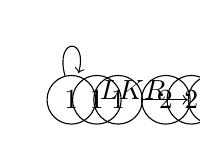
\begin{tikzpicture}  
     \graphbox{$L$}{0mm}{-11mm}{32mm}{15mm}{2mm}{-8mm}{  
         \node[draw,circle]  (x) at (-6mm,0mm) {1};  
        \draw[->] (x) edge[loop above] node  {} (x);

         \node[draw,circle]  (y) at (6mm,0mm) {2};  
       }  
       \graphbox{$K$}{33mm}{-11mm}{32mm}{15mm}{2mm}{-8mm}{  
        \node[draw,circle]  (x) at (-6mm,0mm) {1};  
        \node[draw,circle]  (y) at (6mm,0mm) {2};  
       }  
       \graphbox{$R$}{66mm}{-11mm}{32mm}{15mm}{1mm}{-8mm}{  
        \node[draw,circle]  (x) at (-6mm,0mm) {1};  
        \node[draw,circle]  (y) at (6mm,0mm) {2};  
        \draw[->]  (x) to (y);  
       }    
 \end{tikzpicture}  
 \caption{}
 \label{fig:subgraph_counting:ex_endrullis2024_6d2}
\end{figure}

 Our method can prove its termination with the ruler-graph \tikz[baseline=-0.5ex]{
  \node (x) at (0,0) {$\bullet$};
  \draw[->] (x) edge[loop above] node  {} (x);
} of weight $1$.
\end{example} 

\begin{example}[Limitation]
  \label{ex:plump95_4d1}
 Consider a rule presented in~\cite[Example 4.1]{plump1995ontermination} shown in~\autoref{fig:subgraph_counting:ex_plump95_4d1}.

  \begin{figure}[!htbp]
    \centering
      \resizebox{0.7\textwidth}{!}{
    $\rho = $  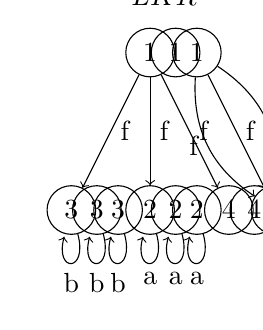
\begin{tikzpicture}[baseline=-20mm]
      \graphbox{$L$}{0mm}{0}{32mm}{40mm}{0}{0}{
          \node[draw,circle]  (n1) at (0,-6mm) {1};
          \node[draw,circle]   (n2) at (0mm,-26mm) {2};
          \node[draw,circle]   (n3) at (-10mm,-26mm) {3};
          \node[draw,circle]   (n4) at (10mm,-26mm) {4};
          \draw[->]  (n2) edge [loop below] node  {a} (n2);
          \draw[->]  (n3) edge [loop below] node  {b} (n3);
          \draw[->]  (n1) to node [right] {f} (n2) ;
          \draw[->]  (n1) to node [right] {f}  (n3);
          \draw[->]  (n1) to node [right] {f}  (n4);
        }
        \graphbox{$K$}{33mm}{0}{32mm}{40mm}{0}{-0}{
          \node[draw,circle]  (n1) at (0,-6mm) {1};
          \node[draw,circle]   (n2) at (0mm,-26mm) {2};
          \node[draw,circle]   (n3) at (-10mm,-26mm) {3};
          \node[draw,circle]   (n4) at (10mm,-26mm) {4};
          \draw[->]  (n2) edge [loop below] node  {a} (n2);
          \draw[->]  (n3) edge [loop below] node  {b} (n3);
        }
        \graphbox{$R$}{66mm}{0}{32mm}{40mm}{0}{-0}{
          \node[draw,circle]  (n1) at (0,-6mm) {1};
          \node[draw,circle]   (n2) at (0mm,-26mm) {2};
          \node[draw,circle]   (n3) at (-10mm,-26mm) {3};
          \node[draw,circle]   (n4) at (10mm,-26mm) {4};
          \draw[->]  (n2) edge [loop below] node  {a} (n2);
          \draw[->]  (n3) edge [loop below] node  {b} (n3);
          \draw[->]  (n1) edge [bend left] node [right] {f} (n4) ;
          \draw[->]  (n1) edge [bend right] node [left] {f}  (n4);
          \draw[->]  (n1) to node [right] {f}  (n4);
        }   
  \end{tikzpicture}
      }
    \caption{}
    \label{fig:subgraph_counting:ex_plump95_4d1}
  \end{figure}
\noindent
\begin{minipage}{0.7\textwidth}
  To prove its termination with our method, a ruler-graph $X$ containing an edge labeled by $f$ must be used, because the number of occurrences of every graph containing only edges labeled by $a$ and $b$ does not change by any rewriting step using $\rho$. But in this case, condition~\eqref{def:non_increasing_rule_img_edges_distinct} of~\autoref{subgraph_counting:def:creates_more_x_on_the_left} cannot be satisfied.
\end{minipage}
\begin{minipage}{0.3\textwidth}
  \hfill
\begin{center}
  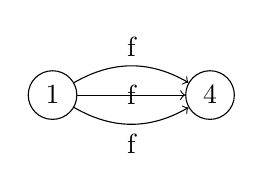
\begin{tikzpicture} 
      \graphbox{}{0}{0}{30mm}{20mm}{-10mm}{-10mm}{
          \node[draw,circle]  (n1) at (0,0mm) {1};
          % \node[draw,circle]   (n2) at (0mm,-26mm) {2};
          % \node[draw,circle]   (n3) at (-10mm,-26mm) {3};
          \node[draw,circle]   (n4) at (20mm,0mm) {4};
          % \draw[->]  (n2) edge [loop below] node  {a} (n2);
          % \draw[->]  (n3) edge [loop below] node  {b} (n3);
          \draw[->]  (n1) edge [bend left] node [above] {f} (n4) ;
          \draw[->]  (n1) edge [bend right] node [below] {f}  (n4);
          \draw[->]  (n1) to node {f}  (n4);
        }  
  \end{tikzpicture}
\end{center}
\end{minipage}

\end{example}

\begin{example}[Limitation]
    \label{ex:endrullis:d3:limitation}  
    Our method fails to prove termination for the rewriting rule from \cite[Example D.3]{endrullis2024generalized_arxiv_v2} shown in~\autoref{fig:subgraph_counting:ex_endrullis_d3_limitation}.
    % because our approach cannot take into account antipatterns(see~\cite[Remark 6.2]{overbeek2024termination_lmcs}).
    This occurs because, for any system $\mathcal{R}$, rewriting step $G \Rightarrow_{\mathcal{R},\mathfrak{M}} H$, set of ruler-graphs $\mathbb{X}$, and weight function $s_\mathbb{X}$, we have $w_{s_\mathbb{X}}(G) \geq w_{s_\mathbb{X}}(H)$ because there exists an injective graph homomorphism from $G$ to $H$.
    
    \begin{figure}[!htbp]
      \centering
        \resizebox{0.7\textwidth}{!}{
    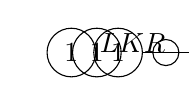
\begin{tikzpicture}  
       \graphbox{$L$}{0mm}{-11mm}{32mm}{15mm}{2mm}{-8mm}{  
           \node[draw,circle]  (x) at (-6mm,0mm) {1};  
           \node[draw,circle]  (y) at (6mm,0mm) {};  
         }  
         \graphbox{$K$}{33mm}{-11mm}{32mm}{15mm}{2mm}{-8mm}{  
           \node[draw,circle]  (x) at (-6mm,0mm) {1};  
         }  
         \graphbox{$R$}{66mm}{-11mm}{32mm}{15mm}{1mm}{-8mm}{  
          \node[draw,circle]  (x) at (-6mm,0mm) {1};  
          \node[draw,circle]  (y) at (6mm,0mm) {};  
          \draw[->]  (x) to (y);  
         }    
   \end{tikzpicture}
        }  
        \caption{}
        \label{fig:subgraph_counting:ex_endrullis_d3_limitation}
    \end{figure}
  \end{example} 

\begin{example}[Limitation]
    \label{ex:overbeek:5d2:limitation}
    Consider a rewriting rule given by Overbeek and Endrullis in~\cite[Example 5.2]{overbeek2024termination_lmcs} shown in~\autoref{fig:subgraph_counting:ex_overbeek_5d2}.
  \begin{figure}[!htbp]
    \centering
    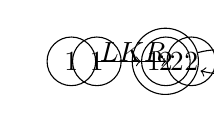
\begin{tikzpicture}
        \graphbox{$L$}{0mm}{-11mm}{32mm}{15mm}{2mm}{-8mm}{
            \node[draw,circle]  (x) at (-6mm,0mm) {1};
            \node[draw,circle]   (y) at (6mm,0mm) {2};
            \draw[->]  (x) to (y);
          }
          \graphbox{$K$}{33mm}{-11mm}{32mm}{15mm}{2mm}{-8mm}{
            \node[draw,circle]  (x) at (-6mm,0mm) {1};
            \node[draw,circle]  (y) at (6mm,0mm) {2};
            \draw[->]  (x) to (y);
          }
          \graphbox{$R$}{66mm}{-11mm}{32mm}{15mm}{1mm}{-8mm}{
            \node[draw,circle]  (x) at (0mm,0mm) {1 2};
            \draw[->]  (x) edge [loop right] (x);
          }  
    \end{tikzpicture} 
    \caption{}
    \label{fig:subgraph_counting:ex_overbeek_5d2}
  \end{figure}
    The termination of this rule is not in the scope of our method due to its non-node-injective right-hand side morphism. It can be proved using the method proposed by Overbeek et al. in~\cite{overbeek2024termination_lmcs}.
\end{example}
 
\begin{example}[Limitation]
  \label{ex:overbeek:5d6_bis:limitation} 
  Consider the DPO rewriting system with monic matches shown in~\autoref{fig:subgraph_counting:ex_overbeek_5d6_bis} from~\cite[Example 5.6]{overbeek2024termination_lmcs} with $\rho$ replaced by $\rho'$.
  \begin{figure}[!htbp]
    \centering
    $\rho' = $\scalebox{0.9} { {
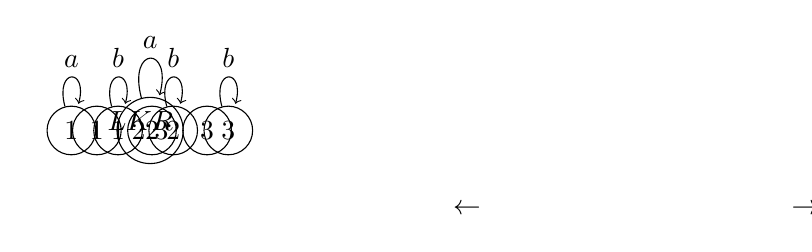
\begin{tikzpicture}[baseline=-10mm]
    \graphbox{$L$}{0mm}{0mm}{38mm}{20mm}{2mm}{-13mm}{
      \node [draw, circle] (x) at (-7mm,0mm) {1};
      \node [draw, circle] (y) at (3mm,0mm) {2 3};
      \draw[->] (x) edge[loop above] node  {$a$} (x);
      \draw[->] (y) edge [loop above] node {$a$} (y);
    }
    \graphbox{$K$}{42mm}{-0mm}{38mm}{20mm}{0mm}{-10mm}{
        \node [draw, circle] (x) at (-7mm,0mm) {1};
        \node [draw, circle] (y) at (0mm,0mm) {2};
        \node [draw, circle] (z) at (7mm,0mm) {3};    
    }
    \begin{scope}[opacity=1]        
    \graphbox{$R$}{85mm}{-0mm}{38mm}{20mm}{2mm}{-13mm}{
      \node [draw, circle] (x) at (-7mm,0mm) {1};
      \node [draw, circle] (y) at (0mm,0mm) {2};
      \node [draw, circle] (z) at (7mm,0mm) {3};
      \draw[->] (x) edge[loop above] node  {$b$} (x);
      \draw[->] (y) edge[loop above] node  {$b$} (y);
      \draw[->] (z) edge[loop above] node  {$b$} (z);
    }
    \end{scope}
    \node () at (40mm,-10mm) {$\leftarrow$};
    \node () at (83mm,-10mm) {$\rightarrow$};
\end{tikzpicture}
}

}
    \caption{}
    \label{fig:subgraph_counting:ex_overbeek_5d6_bis}
  \end{figure} 

  Its termination is not in the scope of our method due to its non-node-injective left-hand side morphism. 
\end{example}